\documentclass[tikz]{standalone}
\usepackage{tikz}

\begin{document}
    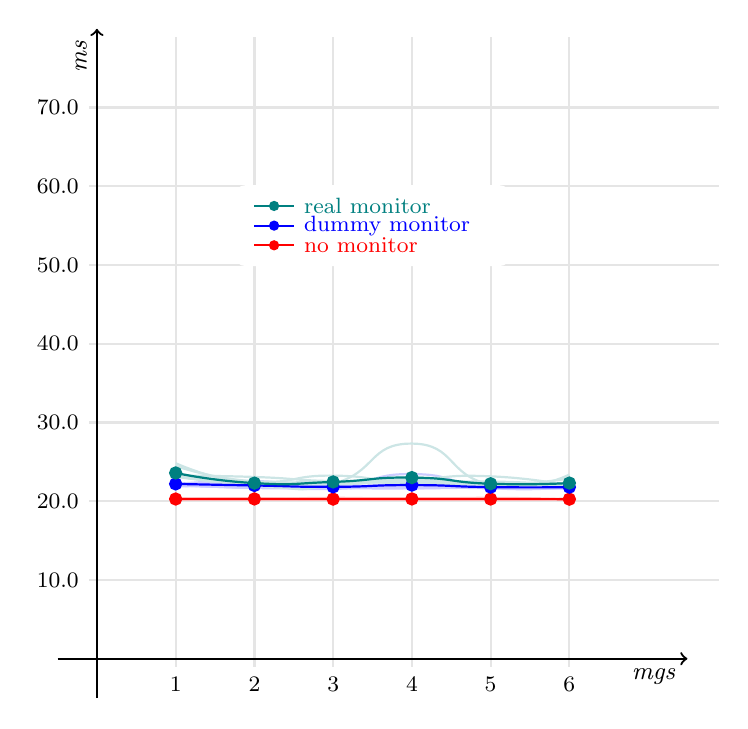
\begin{tikzpicture}[thick]

        % \begin{scope}
        % \clip(-1,18) rectangle ++ (9.5,7.5);

        % \draw[gray!20] (-0.1, 20) node[left, black]{\footnotesize 20} -- (8, 20);
        % \draw[gray!20] (-0.1, 21) node[left, black]{\footnotesize 21} -- (8, 21);
        % \draw[gray!20] (-0.1, 22) node[left, black]{\footnotesize 22} -- (8, 22);
        % \draw[gray!20] (-0.1, 23) node[left, black]{\footnotesize 23} -- (8, 23);
        % \draw[gray!20] (-0.1, 24) node[left, black]{\footnotesize 24} -- (8, 24);

        % \draw[gray!20] (1, 18.9) node[below, black]{\footnotesize 1} -- (1, 25);
        % \draw[gray!20] (2, 18.9) node[below, black]{\footnotesize 2} -- (2, 25);
        % \draw[gray!20] (3, 18.9) node[below, black]{\footnotesize 3} -- (3, 25);
        % \draw[gray!20] (4, 18.9) node[below, black]{\footnotesize 4} -- (4, 25);
        % \draw[gray!20] (5, 18.9) node[below, black]{\footnotesize 5} -- (5, 25);
        % \draw[gray!20] (6, 18.9) node[below, black]{\footnotesize 6} -- (6, 25);

        % \draw[->] (0, 18.5) -- (0, 25) node[above left, rotate=90]{\small \textit{ms}};
        % \draw[->] (-0.5, 19) -- (8, 19) node[below left]{\small \textit{mgs}};

        \foreach \y in {1, 2, ..., 7} {
            \draw[gray!20] (-0.1, \y) node[left, black] {\footnotesize \pgfmathparse{\y*10}\pgfmathresult} -- ++ (8, 0);
        }
        
        
        \foreach \x in {1, 2, ..., 6}{
            \draw[gray!20] (\x, -0.1) node[below, black]{\footnotesize \x} -- ++ (0, 8);
        }

        \draw[->] (0, -0.5) -- ++ (0, 8.5) node[above left, rotate=90]{\small \textit{ms}};
        \draw[->] (-0.5, 0) -- ++ (8, 0) node[below left]{\small \textit{mgs}};

        \draw [red!20!white] plot [smooth, tension=1] coordinates {(1, 2.027) (2, 2.036) (3, 2.023) (4, 2.0260000000000002) (5, 2.02) (6, 2.023) };
        \draw [red!20!white] plot [smooth, tension=1] coordinates {(1, 2.024) (2, 2.0309999999999997) (3, 2.023) (4, 2.024) (5, 2.024) (6, 2.0260000000000002) };
        \draw [red!20!white] plot [smooth, tension=1] coordinates {(1, 2.028) (2, 2.0260000000000002) (3, 2.0300000000000002) (4, 2.029) (5, 2.0260000000000002) (6, 2.028) };
        \draw [red!20!white] plot [smooth, tension=1] coordinates {(1, 2.025) (2, 2.029) (3, 2.024) (4, 2.024) (5, 2.043) (6, 2.02) };
        \draw [red!20!white] plot [smooth, tension=1] coordinates {(1, 2.0309999999999997) (2, 2.022) (3, 2.043) (4, 2.024) (5, 2.0260000000000002) (6, 2.024) };
        \draw [red!20!white] plot [smooth, tension=1] coordinates {(1, 2.029) (2, 2.027) (3, 2.023) (4, 2.032) (5, 2.028) (6, 2.024) };
        \draw [red!20!white] plot [smooth, tension=1] coordinates {(1, 2.036) (2, 2.024) (3, 2.027) (4, 2.032) (5, 2.024) (6, 2.032) };
        \draw [red!20!white] plot [smooth, tension=1] coordinates {(1, 2.0260000000000002) (2, 2.034) (3, 2.024) (4, 2.0260000000000002) (5, 2.028) (6, 2.025) };
        \draw [red!20!white] plot [smooth, tension=1] coordinates {(1, 2.0260000000000002) (2, 2.032) (3, 2.025) (4, 2.032) (5, 2.035) (6, 2.028) };
        \draw [red!20!white] plot [smooth, tension=1] coordinates {(1, 2.024) (2, 2.0309999999999997) (3, 2.0300000000000002) (4, 2.038) (5, 2.024) (6, 2.0300000000000002) };
        
        
        
        \draw [blue!20!white] plot [smooth, tension=1] coordinates {(1, 2.211) (2, 2.185) (3, 2.157) (4, 2.2239999999999998) (5, 2.1670000000000003) (6, 2.177) };
        \draw [blue!20!white] plot [smooth, tension=1] coordinates {(1, 2.2079999999999997) (2, 2.168) (3, 2.1670000000000003) (4, 2.164) (5, 2.189) (6, 2.195) };
        \draw [blue!20!white] plot [smooth, tension=1] coordinates {(1, 2.342) (2, 2.227) (3, 2.183) (4, 2.166) (5, 2.173) (6, 2.1710000000000003) };
        \draw [blue!20!white] plot [smooth, tension=1] coordinates {(1, 2.21) (2, 2.1710000000000003) (3, 2.1870000000000003) (4, 2.198) (5, 2.175) (6, 2.159) };
        \draw [blue!20!white] plot [smooth, tension=1] coordinates {(1, 2.201) (2, 2.2359999999999998) (3, 2.196) (4, 2.19) (5, 2.165) (6, 2.173) };
        \draw [blue!20!white] plot [smooth, tension=1] coordinates {(1, 2.186) (2, 2.205) (3, 2.189) (4, 2.205) (5, 2.184) (6, 2.2039999999999997) };
        \draw [blue!20!white] plot [smooth, tension=1] coordinates {(1, 2.217) (2, 2.256) (3, 2.183) (4, 2.3449999999999998) (5, 2.169) (6, 2.184) };
        \draw [blue!20!white] plot [smooth, tension=1] coordinates {(1, 2.2239999999999998) (2, 2.189) (3, 2.196) (4, 2.184) (5, 2.191) (6, 2.175) };
        \draw [blue!20!white] plot [smooth, tension=1] coordinates {(1, 2.201) (2, 2.178) (3, 2.179) (4, 2.201) (5, 2.1710000000000003) (6, 2.168) };
        \draw [blue!20!white] plot [smooth, tension=1] coordinates {(1, 2.197) (2, 2.185) (3, 2.189) (4, 2.17) (5, 2.206) (6, 2.183) };
        
        
        \draw [teal!20!white] plot [smooth, tension=1] coordinates {(1, 2.352) (2, 2.2190000000000003) (3, 2.246) (4, 2.238) (5, 2.183) (6, 2.195) };
        \draw [teal!20!white] plot [smooth, tension=1] coordinates {(1, 2.359) (2, 2.202) (3, 2.237) (4, 2.227) (5, 2.196) (6, 2.2039999999999997) };
        \draw [teal!20!white] plot [smooth, tension=1] coordinates {(1, 2.321) (2, 2.214) (3, 2.231) (4, 2.2600000000000002) (5, 2.237) (6, 2.199) };
        \draw [teal!20!white] plot [smooth, tension=1] coordinates {(1, 2.448) (2, 2.253) (3, 2.325) (4, 2.228) (5, 2.25) (6, 2.2) };
        \draw [teal!20!white] plot [smooth, tension=1] coordinates {(1, 2.311) (2, 2.243) (3, 2.2489999999999997) (4, 2.2510000000000003) (5, 2.212) (6, 2.2350000000000003) };
        \draw [teal!20!white] plot [smooth, tension=1] coordinates {(1, 2.323) (2, 2.308) (3, 2.255) (4, 2.258) (5, 2.193) (6, 2.2239999999999998) };
        \draw [teal!20!white] plot [smooth, tension=1] coordinates {(1, 2.326) (2, 2.2030000000000003) (3, 2.227) (4, 2.278) (5, 2.316) (6, 2.197) };
        \draw [teal!20!white] plot [smooth, tension=1] coordinates {(1, 2.357) (2, 2.234) (3, 2.247) (4, 2.273) (5, 2.21) (6, 2.289) };
        \draw [teal!20!white] plot [smooth, tension=1] coordinates {(1, 2.4829999999999997) (2, 2.2039999999999997) (3, 2.215) (4, 2.25) (5, 2.21) (6, 2.228) };
        \draw [teal!20!white] plot [smooth, tension=1] coordinates {(1, 2.311) (2, 2.218) (3, 2.223) (4, 2.732) (5, 2.212) (6, 2.339) };
        
        \draw [red] plot [smooth, tension=1, mark=*] coordinates {(1, 2.028)(2, 2.029)(3, 2.027)(4, 2.029)(5, 2.028)(6, 2.026)};
        \draw [blue] plot [smooth, tension=1, mark=*] coordinates {(1, 2.22)(2, 2.2)(3, 2.183)(4, 2.205)(5, 2.179)(6, 2.179)};
        \draw [teal] plot [smooth, tension=1, mark=*] coordinates {(1, 2.359)(2, 2.23)(3, 2.245)(4, 2.3)(5, 2.222)(6, 2.231)};
    

        \coordinate (legend) at (1.75, 5);
        \draw[white, fill=white, rounded corners] (legend) rectangle ++ (3.5, 1);

        \draw[red] ([shift={(0.25, 0.25)}]legend) -- ++ (0.5, 0) node[right]{\footnotesize no monitor};
        \draw[red, fill=red] ([shift={(0.5, 0.25)}]legend) circle (0.05cm);

        \draw[blue] ([shift={(0.25, 0.5)}]legend) -- ++ (0.5, 0) node[right]{\footnotesize dummy monitor};
        \draw[blue, fill=blue] ([shift={(0.5, 0.5)}]legend) circle (0.05cm);

        \draw[teal] ([shift={(0.25, 0.75)}]legend) -- ++ (0.5, 0) node[right]{\footnotesize real monitor};
        \draw[teal, fill=teal] ([shift={(0.5, 0.75)}]legend) circle (0.05cm);

        % \end{scope}
    \end{tikzpicture}
\end{document}